This element simulates a beam-driven monopole mode cavity using the fundamental theorem of beam loading and phasor rotation.
In addition, a generator-driven field may be included using a feedback system \cite{Berenc-IPAC15-MOPMA006}.

Note on phase conventions: the phase convention for the \verb|PHASE_SETPOINT|  parameter of \verb|RFMODE| is the
same as for the \verb|PHASE| parameter of \verb|RFCA|. However, in the output files from \verb|RFMODE|, i.e., the
files requested with the \verb|RECORD| and \verb|FEEDBACK_RECORD| parameters, a different convention is used, which 
differs by $-90$ degrees from the \verb|PHASE_SETPOINT|  parameter. 

The feedback implementation uses either amplitude and phase feedback or else in-phase and quadrature feedback.
Figure \ref{fig:rfFeedbackModel} shows the model used for the feedback system.
More information is available in \cite{Berenc-IPAC15-MOPMA006}.
Feedback is active when a non-zero value is given for \verb|DRIVE_FREQUENCY| and when either
\verb|AMPLITUDE_FILTER| and \verb|PHASE_FILTER| or else
\verb|IN_PHASE_FILTER| and \verb|QUADRATURE_FILTER| are given.

The feedback loop reads the cavity state and acts on the generator at a fixed interval (in buckets) of
\verb|UPDATE_INTERVAL|. 
The timing of this activity is aligned to the arrival time of the first bunch in the \verb|RFMODE| element.
By default (\verb|READ_OFFSET|=0), the timing is such that the state is read just before the next arrival of
that bunch; in particular, it is 180 degrees ahead of that arrival.
If bunches are equally spaced by, say $N_b$ buckets, the \verb|UPDATE_INTERVAL| parameter should ideally be
$m N_b$, where $m>0$ is an integer.
This ensures that the state is read at a fixed timing relative to the bunches.

The rf feedback feature makes use of the voltage amplitude measured when there is no bunch present.
The \verb|RECORD| file shows the voltage seen by the beam, computed by averaging over the voltage for
each particle.
These may deviate by values from a few percent to of order ten percent, depending on the loss factor for the
cavity and the number of bunchess; this is caused by the fact that the rate at which an intense bunch removes
energy from the cavity will typically, albeit briefly, exceed the power from the generator.
To reduce the impact of this effect, one may use the \verb|ADJUSTMENT_FRACTION|, \verb|ADJUSTMENT_START|, and \verb|ADJUSTMENT_INTERVAL|
parameters to modify the voltage setpoint.
If \verb|ADJUSTMENT_FRACTION| is non-zero, then for every \verb|ADJUSTMENT_INTERVAL|$^{th}$ pass after the 
\verb|ADJUSTMENT_START|$^{th}$ pass, the voltage setpoint will be adjusted based on a comparison of the bunch-averaged
voltage to the user's setpoint.
E.g., if the bunch-averaged voltage is 100 V too low and \verb|ADJUSTMENT_FRACTION| is 0.1, the voltage setpoint will
be raised by 10 V.
Users should note that if \verb|ADJUSTMENT_FRACTION| is too large or \verb|ADJUSTMENT_INTERVAL| is too small, the system
may be unstable.

\begin{figure}[htb]
\center
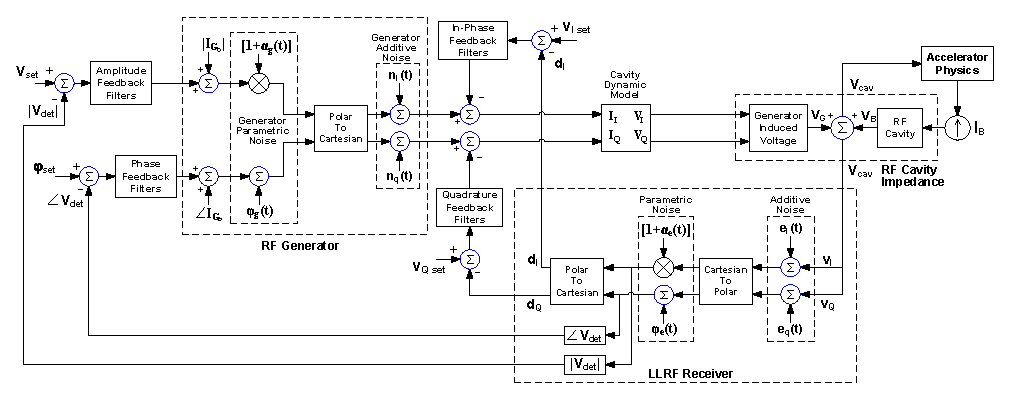
\includegraphics{rfFeedbackModel}
\caption{Rf feedback model used by the {\tt RFMODE} element.}
\label{fig:rfFeedbackModel}
\end{figure}

Normally, the field dumped in the cavity by one particle affects trailing particles in the same turn.
However, if one is also using a \verb|WAKE| or \verb|ZLONGIT| element to simulate the short-range wake of the cavity, this would be double-counting.
In that case, one can use \verb|LONG_RANGE_ONLY=1| to suppress the same-turn effects of the \verb|RFMODE| element.

Two output files are available: the \verb|RECORD| file includes bunch-by-bunch data on the beam-induced fields and the total cavity fields.
The \verb|FEEDBACK_RECORD| file includes tick-by-tick data from the feedback system simulation; {\em writing this file this can significantly impact performance.}

NB: when \verb|BUNCHED_BEAM_MODE| is set to a value other than 1, in order to obtain the effect of several bunches while tracking
only one bunch, the total charge set with the \verb|TOTAL| parameter of the \verb|CHARGE| element should equal the charge in
a single bunch, not the entire beam. However, when \verb|BUNCHED_BEAM_MODE|=1 (allowing an indeterminant number of bunches to be
actually present), then \verb|TOTAL| should be the total for all bunches together.
